\documentclass[11pt,a4paper]{article}

\usepackage[margin=2.2cm]{geometry}
\usepackage{lmodern}
\usepackage[T1]{fontenc}
\usepackage{amsmath}
\usepackage{graphicx}
\usepackage{float}
\usepackage{booktabs}
\usepackage{caption}
\usepackage{enumitem}
\usepackage{tikz}
\usetikzlibrary{arrows.meta,positioning}
\usepackage{hyperref}
\hypersetup{colorlinks=true,linkcolor=black,citecolor=black,urlcolor=blue}

\setlist{itemsep=2pt,topsep=4pt}
\newcommand{\pct}{\,\%}
\newcommand{\file}[1]{\texttt{\detokenize{#1}}}

\title{\textbf{ML-Driven PVT-Variation-Aware}\\ \textbf{Leakage Estimation}}
\author{Digital VLSI Design, Course Project Report\\[2pt]
Team 22 (Madhurbala\_riders): 45nm\_MGK, $V_{DD} = 0.9$\,V, 8-bit parity checker\\[8pt]
Aryan Agrawal (2023102050) \qquad Manikya Pant (2023112024)\\
Vansh Jaiswal (2024102013) \qquad Saarthak Sabharwal (2023102055)}
\date{}

\begin{document}
\sloppy
\maketitle
\vspace{-1.5em}
\begin{center}
Repository: \url{https://github.com/VaNsH-IIIT/dvd-ml-leakage-estimation}
\end{center}

\section{Introduction}

Leakage current sets the static power of a CMOS circuit, and it changes strongly with the supply
voltage, the temperature and the process. Finding it with SPICE for every corner is slow, so the
project asks for machine-learning models that predict it instead. We built them in three steps:

\begin{itemize}
    \item \textbf{Part A, transistors:} ML models of the four terminal currents
    ($I_d$, $I_g$, $I_s$, $I_b$) of one transistor in four cases (NMOS ON, NMOS OFF, PMOS ON,
    PMOS OFF), trained on SPICE data with random $V_{DD}$, temperature, width, terminal voltages
    and process parameters;
    \item \textbf{Part B, gates:} the leakage of INV, NAND2, NOR2, AND2 and OR2 for every input
    combination, computed only from those transistor models, and checked against SPICE of the
    whole gate;
    \item \textbf{Part C, test circuit:} the leakage of our 8-bit parity checker as the sum of its
    gate leakages, checked against SPICE of the full 112-transistor circuit.
\end{itemize}

Figure~\ref{fig:flow} shows the flow. Our final results are a \textbf{0.51\pct\ mean error
(99.49\pct\ mean accuracy)} for both the gates and the parity checker, and 0.12--0.23\pct\
median test error for the transistor models.

\begin{figure}[H]
\centering
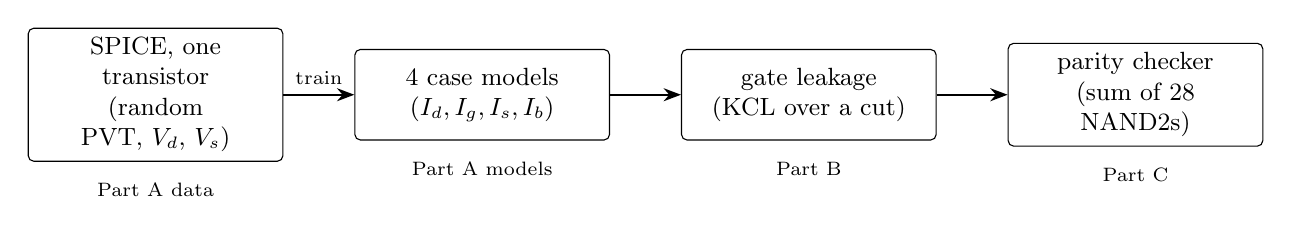
\begin{tikzpicture}[
  box/.style={draw, rounded corners=2pt, align=center, minimum height=1.15cm, text width=3.0cm, font=\small},
  arr/.style={-{Stealth[length=2.2mm]}, thick}]
\node[box] (spice) {SPICE, one transistor\\(random PVT, $V_d$, $V_s$)};
\node[box, right=0.9cm of spice] (ml) {4 case models\\$(I_d, I_g, I_s, I_b)$};
\node[box, right=0.9cm of ml] (gate) {gate leakage\\(KCL over a cut)};
\node[box, right=0.9cm of gate] (circ) {parity checker\\(sum of 28 NAND2s)};
\draw[arr] (spice) -- node[above,font=\scriptsize]{train} (ml);
\draw[arr] (ml) -- (gate);
\draw[arr] (gate) -- (circ);
\node[font=\scriptsize, below=0.15cm of spice] {Part A data};
\node[font=\scriptsize, below=0.15cm of ml] {Part A models};
\node[font=\scriptsize, below=0.15cm of gate] {Part B};
\node[font=\scriptsize, below=0.15cm of circ] {Part C};
\end{tikzpicture}
\caption{Overall flow. Each stage is checked against SPICE of the same transistor, gate or circuit.}
\label{fig:flow}
\end{figure}

We used ngspice-42 for all simulations and Python 3.12 with scikit-learn 1.9.1, LightGBM 4.7.0,
NumPy 2.5.4, SciPy 1.18.1 and pandas 3.0.6 for the models. All results regenerate from the scripts
in \file{scripts/} with fixed seeds; the commands, in order, are in the \file{README.md} of our
repository.

\section{Setup and Choices}

\begin{table}[H]
\centering
\caption{Our assignment and simulation setup.}
\label{tab:setup}
\begin{tabular}{ll}
\toprule
Item & Value \\
\midrule
Model file & \file{45nm_MGK.pm} (PTM, BSIM4 level 54), from the course \file{model.tar} \\
Nominal $V_{DD}$ & 0.9\,V (sampled 0.81--0.99\,V) \\
Channel length, widths & $L = 45$\,nm; $W = 1$--$8 \times L_{min} = 45$--$360$\,nm \\
Test circuit & 8-bit parity checker (7 XOR2 = 28 NAND2, 112 transistors) \\
Simulator & ngspice-42, batch mode, DC operating point (\texttt{op}) \\
Simulator options & \texttt{.options gmin=1e-18 abstol=1e-18 reltol=1e-6 vntol=1e-9} \\
\bottomrule
\end{tabular}
\end{table}

Before generating any data we checked our simulation driver against the professor's sample netlist
\file{22n_NMOS_ON.net}: it reproduces all 48 points to within $4\times10^{-5}$ relative difference
(\file{scripts/verify_sim.py}).

\paragraph{Confirmed with the TAs.}
\begin{itemize}
    \item \textbf{Widths:} $L$ is fixed at 45\,nm and the widths vary between 1 and $8 \times L_{min}$,
    also in the gates and the test circuit.
    \item \textbf{XOR2} for the parity checker is the standard four-NAND2 circuit, since XOR is not
    one of the five gates.
    \item \textbf{Accuracy target:} ``up to 99\pct\ mean accuracy'' means a mean per-sample error
    below 1\pct.
    \item \textbf{Training-set size:} training on more than the 10,000 samples per case is allowed.
    The project's 10,000-row datasets still provide all validation and test rows, and a data-size
    study shows what the 7,000 training rows alone give.
    \item \textbf{Model comparison:} at least four techniques are compared for each transistor case,
    and one final model is kept per case.
\end{itemize}

\paragraph{Our assumptions} (where the document and the TAs' answers leave room):
\begin{itemize}
    \item \textbf{Leakage of a gate or circuit} is all the current drawn from $V_{DD}$-level sources:
    the $V_{DD}$ supply current plus the current drawn by the inputs held at $V_{DD}$, i.e.\ the
    static power divided by $V_{DD}$. The TAs left it to us to work out which currents count.
    Section~\ref{sec:gates} shows what this leakage consists of (gate tunnelling vs sub-threshold and
    junction current), and Section~\ref{sec:parity} shows why the narrower ``$V_{DD}$ pin only''
    definition does not add up to the circuit leakage. We report the total leakage; we did not
    separate the junction current from the sub-threshold current.
    \item \textbf{Widths in a gate or circuit:} the document says all NMOS in a gate share one draw
    and all PMOS share another. We apply this to the widths too: each corner draws one NMOS width
    $W_n$ and one PMOS width $W_p$ (uniform in 45--360\,nm), shared by every NMOS and every PMOS of
    the gate or circuit at that corner.
    \item \textbf{Where the accuracy target applies:} we apply the 1\pct\ mean-error target to the
    leakage estimates of the gates and the circuit, which are the project's outputs. For the
    transistor models we report the median, p95 and mean per current; Section~\ref{sec:models}
    explains why the mean alone is misleading for currents that cross zero.
\end{itemize}

\paragraph{Metrics.} Throughout the report, a sample's error is $|ML - SPICE| / |SPICE|$. We
summarise it by its median, its 95th percentile (p95: 95\pct\ of the samples are at or below it) and
its mean; ``mean accuracy'' $= 100\pct - $ mean error.

\section{Part A: Data Generation}
\label{sec:data}

\paragraph{Sampling} (\file{sim/spec.py}, \file{scripts/a1_generate_data.py}). For each case we draw
10,000 samples independently and uniformly, with a fixed seed per case: $V_{DD}$ in 0.81--0.99\,V
(drawn first), $V_d$ and $V_s$ each in 0--$V_{DD}$, $W$ in 45--360\,nm, $T$ in $-40$ to
125\,\textdegree C, and \texttt{vth0}, \texttt{toxe}, \texttt{ndep}, \texttt{u0} and \texttt{xj}
each at nominal $\pm 10$\pct\ of the 45nm\_MGK card value (NMOS and PMOS drawn separately). The gate
and body voltages $(V_g, V_b)$ are fixed by the case: NMOS ON $(V_{DD}, 0)$, NMOS OFF $(0, 0)$,
PMOS ON $(0, V_{DD})$, PMOS OFF $(V_{DD}, V_{DD})$.

\paragraph{Netlists} (\file{sim/runner.py}). Each sample is one netlist with the model card written
inline with the sample's process values, one MOSFET with $L = 45$\,nm and the sampled $W$, one
voltage source per terminal, the project's \texttt{.options} line, and the sampled temperature.
The terminal currents are ngspice's \texttt{i(Vd)}, \texttt{i(Vg)}, \texttt{i(Vs)} and
\texttt{i(Vb)}, positive when current flows out of the device terminal. The four datasets,
\file{data/partA/<CASE>.csv}, have exactly the project's columns. The 40,000 samples take about
20\,s to simulate on 16 cores.

\paragraph{Split.} Each dataset is split 70/15/15\pct\ (7,000 / 1,500 / 1,500 rows) with seed 22.
For the final models the training part is enlarged with up to 80,000 extra samples per case, drawn
the same way with other seeds (\file{data/partA_extra/}); validation and test always stay the
project's rows. The test rows are never used to choose or tune a model.

\paragraph{Data check} (\file{scripts/a2_check_data.py}). Every row has all values, inside its range.
Kirchhoff's law holds in every row: the four currents balance to within $10^{-15}$\,A or 0.1\pct\ of
the largest current (median residual about $7\times10^{-7}$ of the largest current, from ngspice's
6--7 printed digits). The trends are physical (Figure~\ref{fig:trends}): the OFF current rises
$\times 115$ (NMOS) and $\times 12$ (PMOS) from $-40$ to 125\,\textdegree C, falls as $|$\texttt{vth0}$|$
rises ($\times 0.14$ and $\times 0.33$ over $\pm 10$\pct), and the gate current falls $\times 0.07$ as
\texttt{toxe} rises by 20\pct.

\begin{figure}[H]
\centering
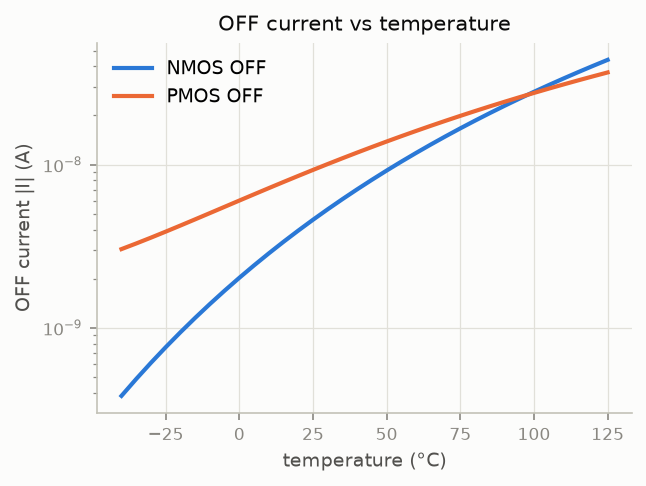
\includegraphics[width=0.32\linewidth]{partA/trend_off_vs_temp.png}\hfill
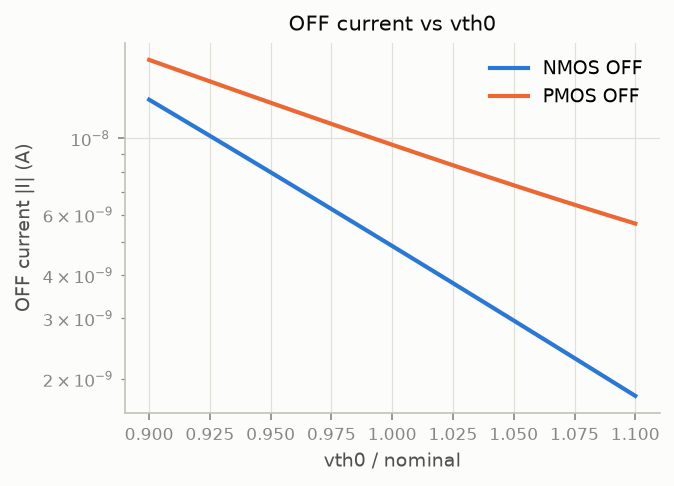
\includegraphics[width=0.33\linewidth]{partA/trend_off_vs_vth0.png}\hfill
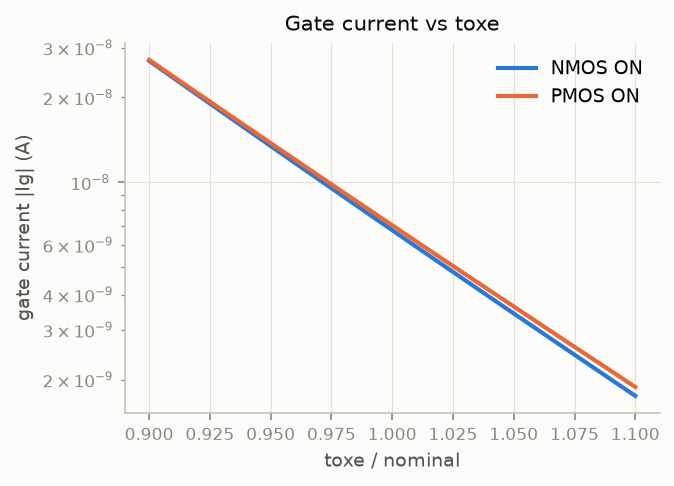
\includegraphics[width=0.33\linewidth]{partA/trend_gate_vs_toxe.png}
\caption{Trend checks, one parameter swept from the nominal point ($W = L_{min}$, $V_{DD} = 0.9$\,V,
27\,\textdegree C). OFF current at $V_{ds} = V_{DD}$; gate current of ON devices at $V_d = V_s$.}
\label{fig:trends}
\end{figure}

\paragraph{Structure in the data that shaped the models.}
\begin{enumerate}
    \item The device is drain/source symmetric: swapping $V_d$ and $V_s$ swaps $I_d$ and $I_s$. If we
    rename the terminals ``hi'' (higher voltage) and ``lo'', three of the four currents of every case
    keep one sign over the whole dataset.
    \item The exception is one terminal per OFF case (lo for NMOS, hi for PMOS), where the outgoing
    channel current and the incoming gate-tunnelling current can cancel. In 8.0\pct\ (NMOS) and
    4.8\pct\ (PMOS) of the OFF rows it is below 3\pct\ of the gate current.
    \item The OFF body current is about $10^{-14}$\,A, nearly constant, and 6--8 decades below the
    gate leakages ($8.8\times10^{-9}$ to $1.7\times10^{-6}$\,A).
\end{enumerate}

\section{Part A: Transistor Models}
\label{sec:models}

\subsection{Preprocessing}

Each sample is rewritten in the hi/lo form above, and predictions are mapped back to $I_d$ and
$I_s$. The model has 17 inputs: $T$ and $1/T$, $V_{DD}$, $W/L$ and $\log(W/L)$, $V_{hi}$, $V_{lo}$,
$V_{hi} - V_{lo}$ and its $\log_{10}$, $V_g - V_{hi}$, $V_g - V_{lo}$, $V_b - V_{lo}$, and the five
process deviations, all standardised. The currents span 7--10 decades, so each target is
$\operatorname{asinh}(I / I_0)$, which behaves like log-current: a fixed error in the target is a
fixed relative error in the current, and it is smooth through zero.
\begin{itemize}
    \item For the fixed-sign currents, $I_0 = 10^{-3} \times$ the median $|I|$ of the training set.
    \item For the mixed-sign OFF terminal, $I_0 = 0.1\,|I_g|$ of the same sample (at prediction time,
    the model's own $I_g$ prediction), so its zero crossing becomes a gentle slope. This cut that
    terminal's validation error about threefold (Section~\ref{sec:errors}).
\end{itemize}
One regressor is trained per current. A saved case model (\file{trained_models/<CASE>.joblib}) maps
the project's input columns to $(I_d, I_g, I_s, I_b)$.

\subsection{Comparison of four techniques}

We compared four model types on each case (\file{ml/models.py}, \file{scripts/a3_compare_models.py}):
\begin{enumerate}
    \item \textbf{Polynomial:} degree-3 polynomial features + ridge regression ($\alpha = 10^{-4}$);
    \item \textbf{LightGBM:} 4,000 trees, learning rate 0.03, 63 leaves, at least 10 rows per leaf,
    row and column subsampling 0.8;
    \item \textbf{MLP:} 3 hidden layers $\times$ 128 tanh units, Adam with learning rate
    $2\times10^{-3}$, L2 penalty $10^{-6}$, early stopping on 10\pct\ of the training rows
    (patience 200 epochs);
    \item \textbf{Gaussian process (GP):} ARD RBF kernel (one length scale per input) $\times$
    constant + white noise; kernel fitted on 1,000 training rows, then conditioned on all of them.
\end{enumerate}

\begin{table}[H]
\centering
\caption{Model comparison on the validation set, 7,000 training rows: $R^2$ of the worst of the
four currents (on the asinh target), and median / p95 error pooled over the four currents. Bold:
lowest p95 per case.}
\label{tab:compare}
\small
\begin{tabular}{llllll}
\toprule
Case & Metric & Polynomial & LightGBM & MLP & Gaussian process \\
\midrule
NMOS ON  & $R^2$ & 0.9840 & 0.9979 & 0.9995 & 0.9989 \\
         & median / p95 & 8.72 / 56.7\pct & 3.16 / 26.8\pct & \textbf{0.43 / 2.58\pct} & 0.11 / 3.99\pct \\
\addlinespace
NMOS OFF & $R^2$ & 0.920 & 0.923 & 0.898 & 0.902 \\
         & median / p95 & 7.98 / 84.5\pct & 2.31 / 31.2\pct & \textbf{1.06 / 10.5\pct} & 0.53 / 15.8\pct \\
\addlinespace
PMOS ON  & $R^2$ & 0.9891 & 0.9982 & 0.9999 & 0.9986 \\
         & median / p95 & 5.51 / 29.5\pct & 2.53 / 19.2\pct & 0.41 / 2.13\pct & \textbf{0.07 / 1.47\pct} \\
\addlinespace
PMOS OFF & $R^2$ & 0.875 & 0.891 & 0.853 & 0.905 \\
         & median / p95 & 8.81 / 86.3\pct & 2.26 / 29.9\pct & \textbf{1.04 / 8.45\pct} & 0.29 / 10.7\pct \\
\bottomrule
\end{tabular}
\end{table}

The polynomial is too stiff for 17 inputs and many decades of current, and the trees predict in
steps, which does not suit a smooth function that has to be within 1\pct. The GP has the best median
in every case, but a heavy tail: one smooth kernel cannot follow the steep regions, and it falls back
towards the mean at the edges of the input box. The MLP has the lowest p95 in three of the four cases.
The lower $R^2$ in the OFF cases comes from the body current, which is $\sim\!10^{-14}$\,A and nearly
constant, so its $R^2$ says little; the other three OFF currents have $R^2 \geq 0.9996$ for the MLP.

\paragraph{Choice rule:} lowest validation p95, then lowest median. We choose on the tail rather than
the median because the gates put transistors at the edges of the training box; the GP shows why (it
gives 12.6\pct\ median error at gate level, Section~\ref{sec:limits}). No gate or circuit result is
used to train or choose a model.

\subsection{More data and ensembles}

\paragraph{Data size.} We retrained the MLP on less and more data. Validation and test stay on the
project's dataset.

\begin{table}[H]
\centering
\caption{MLP validation median / p95 error vs training rows.}
\label{tab:size}
\small\setlength{\tabcolsep}{4pt}
\begin{tabular}{llllll}
\toprule
Case & 2,000 & 4,000 & 7,000 & 27,000 & 47,000 \\
\midrule
NMOS ON  & 0.75 / 7.56\pct & 0.67 / 4.49\pct & 0.43 / 2.58\pct & 0.31 / 1.38\pct & 0.32 / 1.47\pct \\
NMOS OFF & 1.44 / 16.7\pct & 0.81 / 10.4\pct & 1.06 / 10.5\pct & 0.71 / 6.96\pct & 0.71 / 7.66\pct \\
PMOS ON  & 1.00 / 7.60\pct & 0.46 / 2.51\pct & 0.41 / 2.13\pct & 0.34 / 1.42\pct & 0.32 / 1.29\pct \\
PMOS OFF & 1.19 / 14.9\pct & 0.68 / 10.1\pct & 1.04 / 8.45\pct & 0.58 / 8.14\pct & 0.64 / 7.36\pct \\
\bottomrule
\end{tabular}
\end{table}

At 2,000 rows every case is clearly worse. Above 7,000 rows the tail improves up to 27,000 rows,
after which a single network levels off: its remaining error is mostly run-to-run variance. More
data costs little simulation time (about 20\,s for 40,000 samples) but longer training (1--2.4\,h per
case for one 87,000-row ensemble).

\paragraph{Ensembles.} Averaging three MLPs trained with different seeds removes most of that
variance. We trained three ensemble variants on 87,000 rows, which differ in what the networks learn:
\begin{itemize}
    \item \textbf{per-width targets:} current $/\,(W/L)$, since leakage scales almost linearly with width;
    \item \textbf{plain-current targets:} the current itself;
    \item \textbf{linear baseline:} a ridge fit first, with the networks learning only what it leaves.
    Log-current is close to linear in most inputs, and the linear part carries those trends into the
    corners of the input box, where training rows are sparse.
\end{itemize}
Their errors are partly independent, so we also scored equal-weight averages of their predicted
currents (Table~\ref{tab:ens}).

\begin{table}[H]
\centering
\caption{Validation median / p95 error, 87,000 training rows. Bold: chosen per case.}
\label{tab:ens}
\small\setlength{\tabcolsep}{4pt}
\begin{tabular}{lllll}
\toprule
Candidate & NMOS ON & NMOS OFF & PMOS ON & PMOS OFF \\
\midrule
Ensemble, per-width targets & 0.18 / 0.87\pct & 0.44 / 4.96\pct & 0.18 / 0.71\pct & 0.38 / 4.59\pct \\
Ensemble, plain-current targets & 0.20 / 0.92\pct & 0.30 / 4.02\pct & 0.20 / 0.80\pct & 0.40 / 4.49\pct \\
Ensemble, linear baseline & 0.18 / 0.91\pct & 0.31 / 3.52\pct & 0.18 / 0.87\pct & 0.29 / 4.44\pct \\
Average, plain-current + linear & 0.15 / 0.68\pct & \textbf{0.24 / 3.05\pct} & 0.14 / 0.62\pct & 0.25 / 3.48\pct \\
Average of all three & \textbf{0.13 / 0.60\pct} & 0.23 / 3.22\pct & \textbf{0.12 / 0.52\pct} & \textbf{0.22 / 3.40\pct} \\
\bottomrule
\end{tabular}
\end{table}

So the final model of each case is an MLP ensemble: the average of all three variants for NMOS ON,
PMOS ON and PMOS OFF, and of the plain-current and linear-baseline variants for NMOS OFF.

\subsection{Final models on the test set}

\begin{table}[H]
\centering
\caption{Chosen models on the 1,500 test rows per case, errors pooled over the four currents, and
median / p95 error per current. $^{*}$Mean over the currents with $|I| \geq 10^{-11}$\,A only.}
\label{tab:test}
\small\setlength{\tabcolsep}{4pt}
\begin{tabular}{llllllll}
\toprule
Case & Median & p95 & Mean & Mean$^{*}$ & $I_d$ & $I_g$ & $I_b$ \\
\midrule
NMOS ON  & 0.13\pct & 0.61\pct & 24.1\pct & 3.03\pct & 0.12 / 0.7 & 0.12 / 0.7 & 0.14 / 0.5 \\
NMOS OFF & 0.23\pct & 3.16\pct & 2.15\pct & 0.36\pct & 0.22 / 1.3 & 0.16 / 0.5 & 0.51 / 22.0 \\
PMOS ON  & 0.12\pct & 0.53\pct & 0.40\pct & 0.43\pct & 0.13 / 0.5 & 0.11 / 0.6 & 0.13 / 0.5 \\
PMOS OFF & 0.22\pct & 3.05\pct & 3.28\pct & 0.29\pct & 0.19 / 1.0 & 0.14 / 0.5 & 0.82 / 20.0 \\
\bottomrule
\end{tabular}
\end{table}

\begin{itemize}
    \item Test and validation agree to within 0.01\pct\ in the median, so there is no sign of
    over-fitting to the validation split. ($I_s$ behaves like $I_d$; all numbers are in
    \file{reports/partA/MODELS.md}.)
    \item In the OFF cases the p95 comes almost entirely from the $\sim\!10^{-14}$\,A body current.
    The three currents that matter have p95 $\leq 1.4$\pct.
    \item The means are pulled up by a few near-zero currents. In NMOS ON, when $V_d \approx V_s$ the
    channel current crosses zero ($|I_d|$ down to $1.6\times10^{-12}$\,A against $\sim\!10^{-4}$\,A
    at full bias); one such sample alone is 78,000\pct\ off, with an absolute error of only
    $10^{-9}$\,A. These channel currents never enter the gate leakage (Section~\ref{sec:gates}).
\end{itemize}

\begin{figure}[H]
\centering
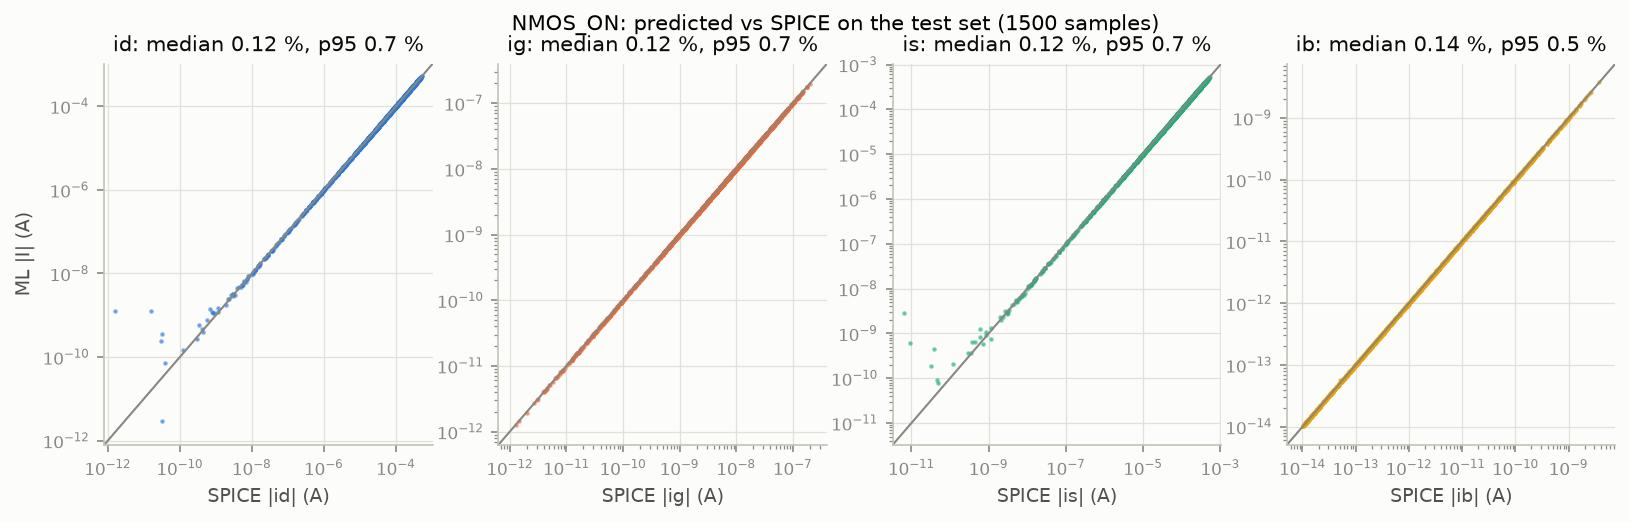
\includegraphics[width=0.49\linewidth]{partA/pred_vs_spice_NMOS_ON.png}\hfill
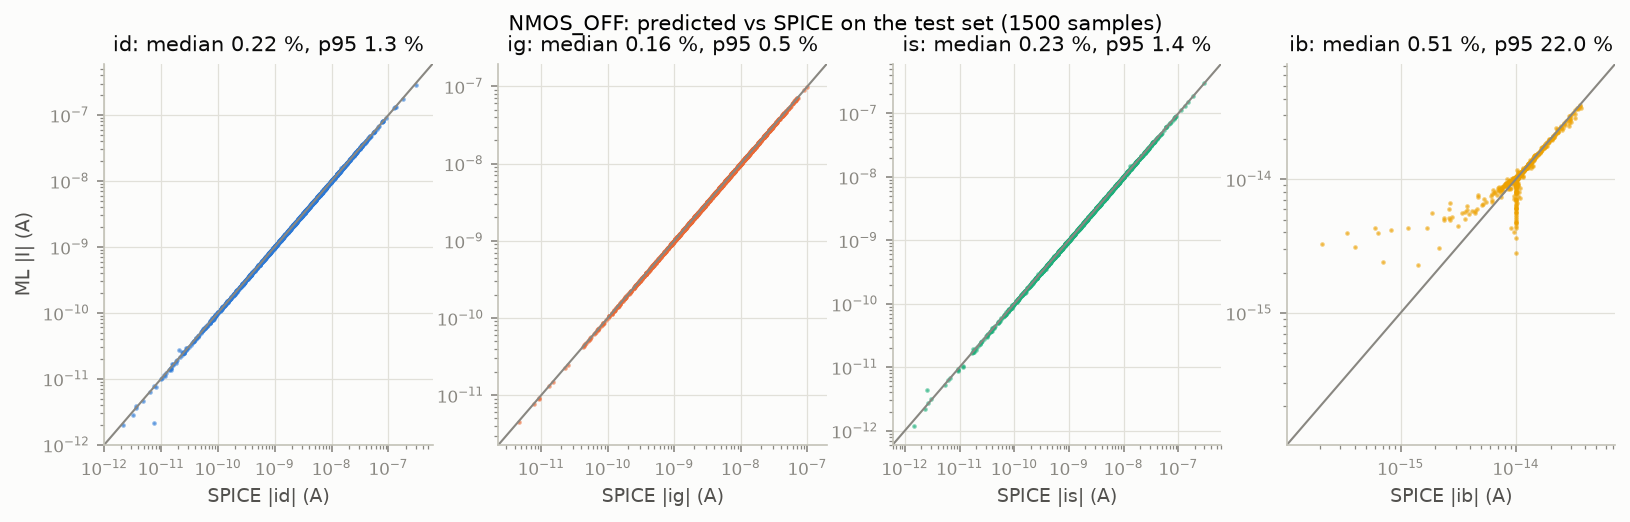
\includegraphics[width=0.49\linewidth]{partA/pred_vs_spice_NMOS_OFF.png}\\[4pt]
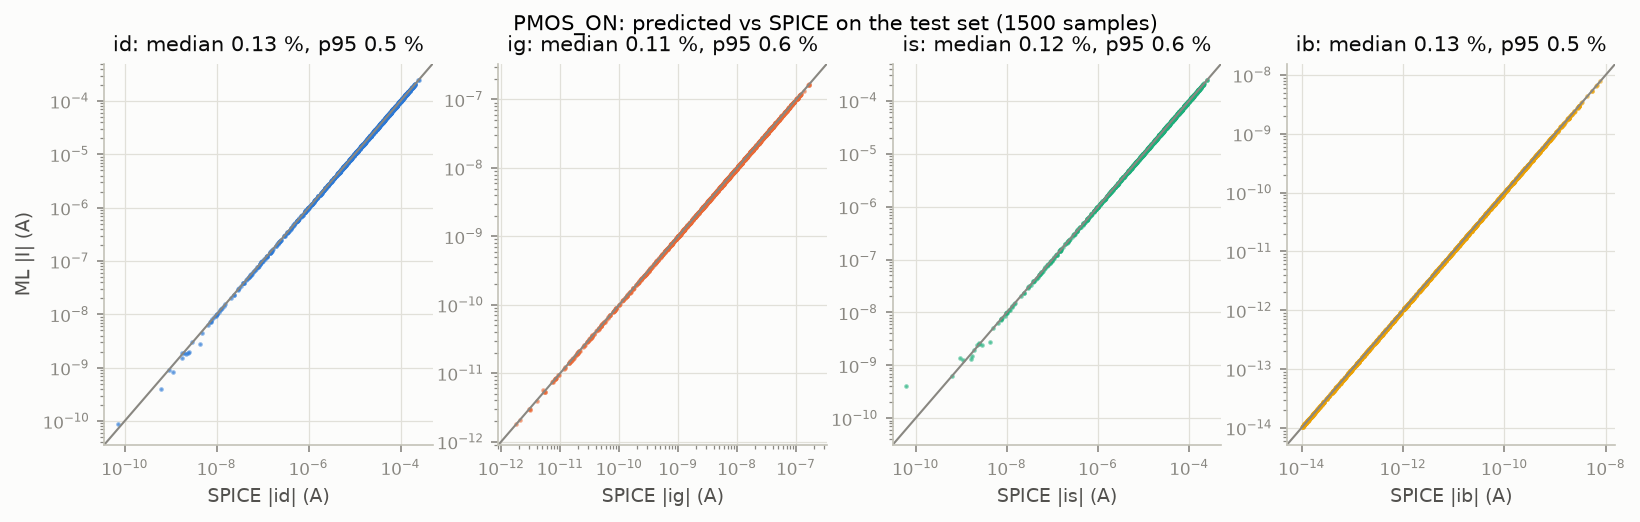
\includegraphics[width=0.49\linewidth]{partA/pred_vs_spice_PMOS_ON.png}\hfill
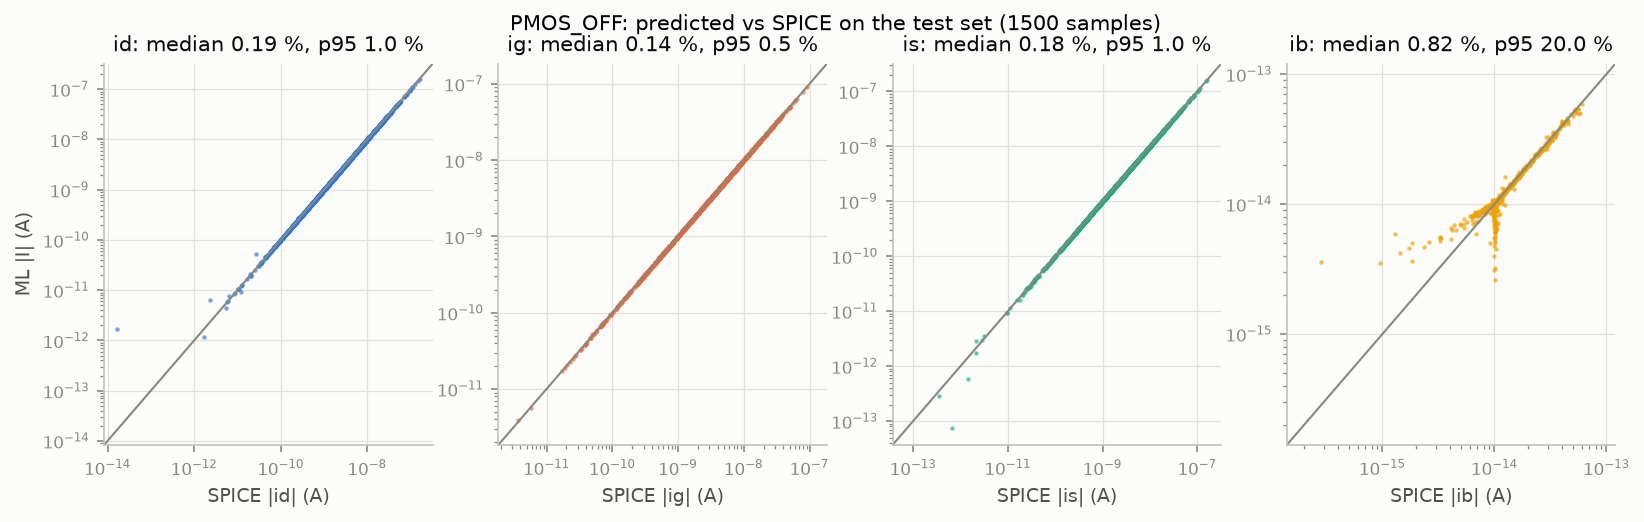
\includegraphics[width=0.49\linewidth]{partA/pred_vs_spice_PMOS_OFF.png}
\caption{Chosen models on the test set: predicted vs SPICE $|I|$ for each terminal current.}
\label{fig:pred}
\end{figure}

\section{Part B: Gate Leakage}
\label{sec:gates}

\paragraph{Gates} (\file{sim/gates.py}, \file{scripts/b1_gates_spice.py}). We used standard static
CMOS gates, with AND2/OR2 = NAND2/NOR2 + INV. Each gate was simulated for every input combination at
200 corners, each with its own $V_{DD}$, $T$, NMOS and PMOS process draws, and widths $W_n$ and $W_p$:
3,600 simulations in total. The inputs are at exactly 0 or $V_{DD}$.

\paragraph{What is the leakage made of?} We repeated every gate simulation with the model's gate
tunnelling switched off (\texttt{igcmod = igbmod = 0}, \file{scripts/b3_leakage_components.py}).
What remains is sub-threshold plus junction current.

\begin{table}[H]
\centering
\caption{Make-up of the gate leakage (medians over the 200 corners).}
\label{tab:components}
\small
\begin{tabular}{lllll}
\toprule
Gate, inputs & SPICE leakage (A) & Gate tunnelling & Sub-threshold & Drawn through \\
 & & & + junction & inputs at $V_{DD}$ \\
\midrule
INV 0 / 1 & 1.10e-7 / 1.13e-7 & 65 / 46\pct & 35 / 54\pct & 0 / 46\pct \\
NAND2 00 / 11 & 1.01e-7 / 2.26e-7 & 97 / 46\pct & 3 / 54\pct & 0 / 46\pct \\
NOR2 00 / 11 & 2.19e-7 / 8.97e-8 & 64 / 92\pct & 36 / 8\pct & 0 / 92\pct \\
All 3,600 runs & & 67\pct & 33\pct & \\
\bottomrule
\end{tabular}
\end{table}

With the 0.9\,nm oxide of this model card, gate tunnelling is about two thirds of the leakage. Sub-threshold
current grows with temperature and takes over when hot: the tunnelling share falls from 89\pct\
below 0\,\textdegree C to 34\pct\ above 85\,\textdegree C. When inputs are high, a large part of the
leakage (up to 92\pct\ for NOR2 11) is gate tunnelling into the ON NMOS channels, drawn through those
inputs. That is why our leakage counts the input currents.

\subsection{ML gate leakage}

For each gate and corner (\file{ml/gate_eval.py}, \file{scripts/b2_gates_ml.py}):
\begin{enumerate}
    \item each transistor's terminal voltages come from the SPICE node voltages, with exact inputs and rails;
    \item its case (ON/OFF) follows from its gate voltage, and that case's model predicts its four currents;
    \item the currents are combined into the $V_{DD}$ current by Kirchhoff's law over a
    \textbf{cut through the OFF devices};
    \item the current drawn by each input held at $V_{DD}$ (the gate currents of the transistors it
    drives) is added.
\end{enumerate}

\paragraph{Why a cut through the OFF devices?} Summing the currents at the $V_{DD}$ node needs the
channel current of the ON pull-up transistors. These sit at a $V_{ds}$ of microvolts, where their
current is a tiny difference set by the OFF network, and the training data has almost no rows there.
But Kirchhoff's law holds for any set of nodes $S$ that contains $V_{DD}$ (and not ground or an
input): $I_{leak} = -\sum$ of the terminal currents at the nodes in $S$. For a device with both drain
and source inside $S$, $I_d + I_s = -(I_g + I_b)$, so its channel current cancels exactly. We pick
the $S$ whose boundary devices are all OFF, with the largest $|V_{ds}|$. With every transistor
simulated alone in SPICE instead of the ML model, this recipe reproduces the full-gate SPICE leakage
to within 0.0005\pct, so the recipe is exact and the remaining error belongs to the models.

\begin{table}[H]
\centering
\caption{How the currents are combined, same models, all 3,600 gate simulations.}
\label{tab:cut}
\begin{tabular}{llll}
\toprule
Method & Median & p95 & Mean \\
\midrule
Sum at the $V_{DD}$ node & 2.43\pct & 18.2\pct & 5.17\pct \\
Minimal supernode ($V_{DD}$ + ON-connected nodes) & 0.38\pct & 1.37\pct & 0.52\pct \\
\textbf{Best cut through the OFF devices (used)} & \textbf{0.37\pct} & \textbf{1.33\pct} & \textbf{0.51\pct} \\
\bottomrule
\end{tabular}
\end{table}

\subsection{Results}

\begin{table}[H]
\centering
\caption{Gate leakage, ML vs SPICE, 200 corners per row. Bias = median of ML/SPICE $- 1$.}
\label{tab:gates}
\small
\begin{tabular}{llllllll}
\toprule
Gate & Inputs & SPICE median (A) & ML median (A) & Bias & Median error & p95 error \\
\midrule
INV & 0 & 1.098e-07 & 1.097e-07 & +0.26\pct & 0.50\pct & 1.66\pct \\
INV & 1 & 1.129e-07 & 1.125e-07 & $-$0.28\pct & 0.48\pct & 1.35\pct \\
\addlinespace
NAND2 & 00 & 1.008e-07 & 1.016e-07 & +0.53\pct & 0.57\pct & 1.43\pct \\
NAND2 & 01 & 1.579e-07 & 1.586e-07 & +0.10\pct & 0.34\pct & 1.18\pct \\
NAND2 & 10 & 9.068e-08 & 9.085e-08 & +0.29\pct & 0.44\pct & 1.47\pct \\
NAND2 & 11 & 2.256e-07 & 2.250e-07 & $-$0.23\pct & 0.43\pct & 1.35\pct \\
\addlinespace
NOR2 & 00 & 2.189e-07 & 2.188e-07 & +0.27\pct & 0.48\pct & 1.54\pct \\
NOR2 & 01 & 1.668e-07 & 1.664e-07 & +0.06\pct & 0.29\pct & 1.38\pct \\
NOR2 & 10 & 9.702e-08 & 9.693e-08 & $-$0.21\pct & 0.43\pct & 1.55\pct \\
NOR2 & 11 & 8.966e-08 & 8.930e-08 & $-$0.33\pct & 0.48\pct & 1.43\pct \\
\addlinespace
AND2 & 00 & 2.420e-07 & 2.419e-07 & +0.13\pct & 0.30\pct & 1.10\pct \\
AND2 & 01 & 2.823e-07 & 2.823e-07 & $-$0.17\pct & 0.30\pct & 1.16\pct \\
AND2 & 10 & 2.128e-07 & 2.127e-07 & $-$0.12\pct & 0.27\pct & 1.18\pct \\
AND2 & 11 & 3.466e-07 & 3.457e-07 & $-$0.12\pct & 0.28\pct & 1.01\pct \\
\addlinespace
OR2 & 00 & 3.478e-07 & 3.475e-07 & $-$0.21\pct & 0.38\pct & 1.27\pct \\
OR2 & 01 & 2.875e-07 & 2.874e-07 & +0.12\pct & 0.32\pct & 1.05\pct \\
OR2 & 10 & 2.230e-07 & 2.233e-07 & +0.00\pct & 0.28\pct & 1.01\pct \\
OR2 & 11 & 2.299e-07 & 2.296e-07 & $-$0.02\pct & 0.28\pct & 1.33\pct \\
\midrule
\multicolumn{5}{l}{\textbf{All 3,600 simulations} (mean error \textbf{0.51\pct}, 99.49\pct\ mean accuracy)} & \textbf{0.37\pct} & \textbf{1.33\pct} \\
\bottomrule
\end{tabular}
\end{table}

89\pct\ of the gate simulations are within 1\pct, and only 0.33\pct\ exceed 5\pct\ (largest 6.9\pct).

\begin{itemize}
    \item \textbf{Most accurate: AND2 and OR2} (0.27--0.38\pct\ median). Their leakage is the sum of two
    stages whose device errors partly offset.
    \item \textbf{Least accurate: the output-high cases NAND2 00 (0.57\pct) and INV 0 (0.50\pct).} Their
    leakage flows through OFF NMOS with the drain at $V_{DD}$, and includes the gate tunnelling of the
    ON PMOS at $V_d \approx V_s \approx V_{DD}$; both are at edges of the training data.
    \item \textbf{The bias is small} ($-0.33$ to $+0.53$\pct), so the error is mainly scatter.
\end{itemize}

\begin{figure}[H]
\centering
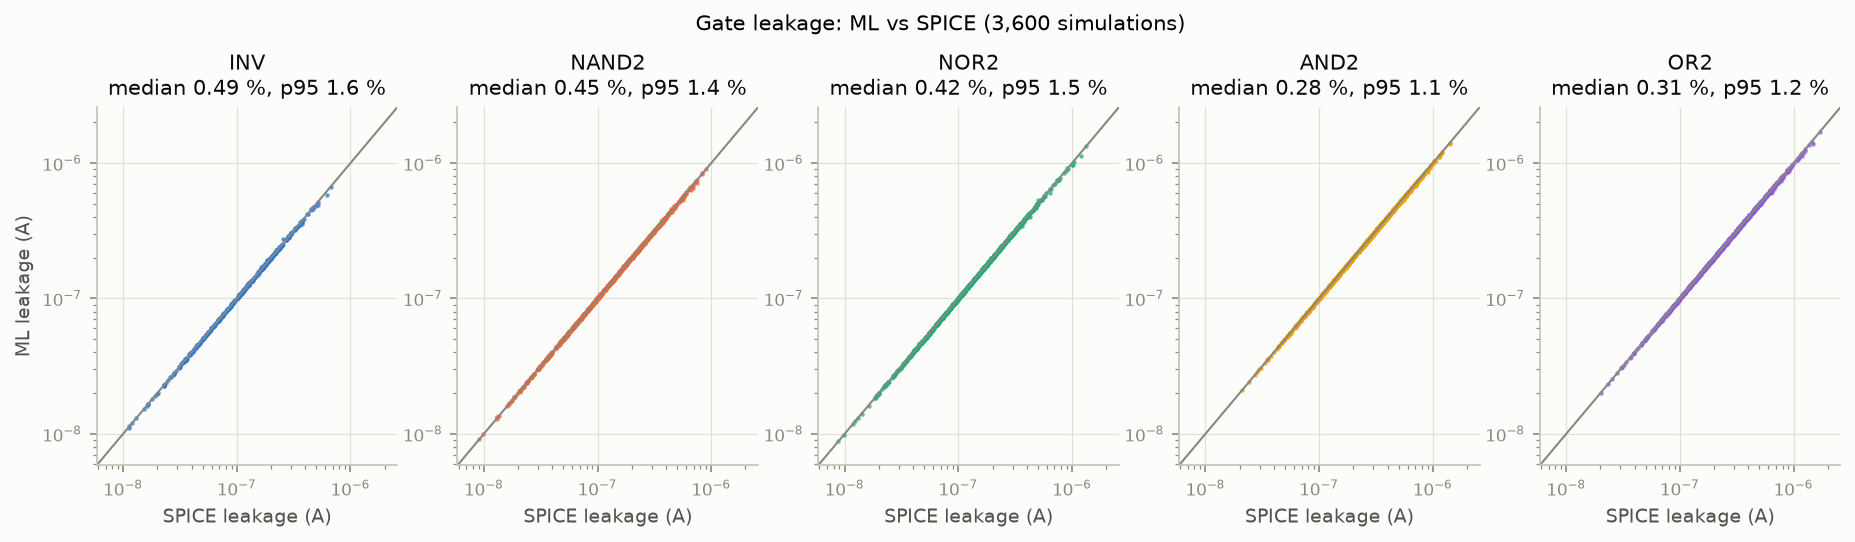
\includegraphics[width=\linewidth]{partB/gates_parity.png}
\caption{Gate leakage, ML vs SPICE, all 3,600 gate simulations (log axes), one panel per gate.}
\label{fig:gates}
\end{figure}

\paragraph{Internal node voltages.} We also solved Kirchhoff's law at each internal node with the ML
models. The ML node voltages agree with SPICE to a median of 0.33\,mV or better in every gate case,
but fail in a few corners where the balance depends on an ON device at microvolt $V_{ds}$ (worst:
OR2 inputs 10, node y, 0.77\,V).

\paragraph{How the gate results were used.} No gate or circuit result was used to train or select a
model. The gate runs did shape the method: the cut-based sum, the ensembles and the three ensemble
variants were developed after gate runs showed where the earlier models were weak. So, to check the
numbers on data that influenced nothing, \file{scripts/d3_fresh_check.py} draws new transistor samples
and 100 new corners with fresh seeds. The gates give 0.37\pct\ median and \textbf{0.50\pct\ mean}
error there, the same as above.

\section{Part C: 8-bit Parity Checker}
\label{sec:parity}

\paragraph{Circuit} (\file{sim/parity.py}). Seven XOR2 gates in a tree compute the parity of the 8
inputs, and each XOR2 is the standard four-NAND2 circuit (Figure~\ref{fig:parity}): 28 NAND2 and 112
transistors. SPICE simulates the full netlist for all 256 input vectors at the same 200 corners:
51,200 runs, about 4.5 minutes.

\begin{figure}[H]
\centering
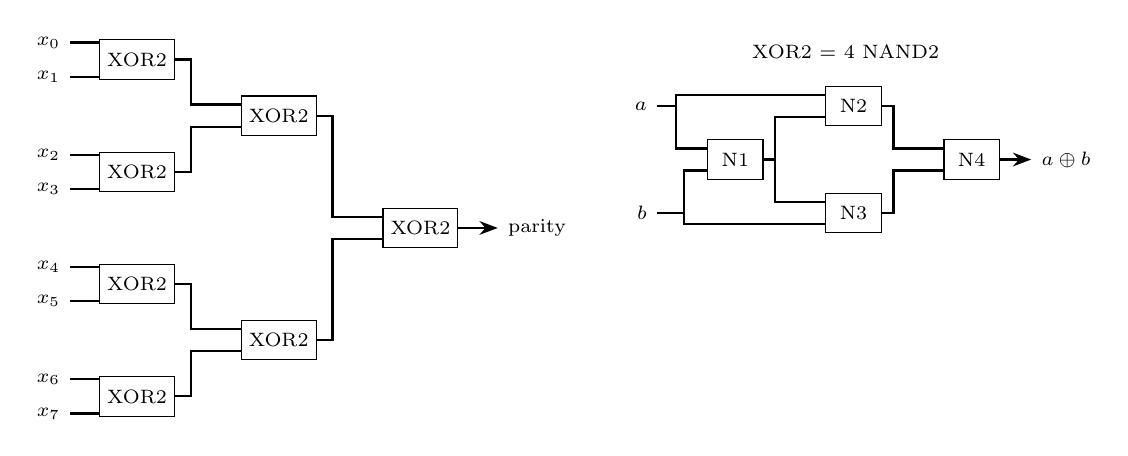
\begin{tikzpicture}[
  x=1cm, y=0.62cm,
  g/.style={draw, minimum width=0.95cm, minimum height=0.5cm, font=\scriptsize, inner sep=1pt},
  n/.style={draw, minimum width=0.7cm, minimum height=0.5cm, font=\scriptsize, inner sep=1pt},
  w/.style={thick}]
% XOR tree
\foreach \i in {0,...,3} {
  \node[g] (a\i) at (0, 5.5-2*\i*1.15) {XOR2};
  \node[font=\scriptsize, anchor=east] at (-0.85, 5.5-2*\i*1.15+0.35) {$x_{\the\numexpr2*\i\relax}$};
  \node[font=\scriptsize, anchor=east] at (-0.85, 5.5-2*\i*1.15-0.35) {$x_{\the\numexpr2*\i+1\relax}$};
  \draw[w] (-0.85, 5.5-2*\i*1.15+0.35) -- ++(0.37,0);
  \draw[w] (-0.85, 5.5-2*\i*1.15-0.35) -- ++(0.37,0);
}
\node[g] (b0) at (1.8, 4.35) {XOR2};
\node[g] (b1) at (1.8, -0.25) {XOR2};
\node[g] (c0) at (3.6, 2.05) {XOR2};
\draw[w] (a0.east) -- ++(0.2,0) |- ([yshift=4pt]b0.west);
\draw[w] (a1.east) -- ++(0.2,0) |- ([yshift=-4pt]b0.west);
\draw[w] (a2.east) -- ++(0.2,0) |- ([yshift=4pt]b1.west);
\draw[w] (a3.east) -- ++(0.2,0) |- ([yshift=-4pt]b1.west);
\draw[w] (b0.east) -- ++(0.2,0) |- ([yshift=4pt]c0.west);
\draw[w] (b1.east) -- ++(0.2,0) |- ([yshift=-4pt]c0.west);
\draw[w,-{Stealth}] (c0.east) -- ++(0.5,0) node[right, font=\scriptsize] {parity};
% XOR2 from 4 NAND2
\begin{scope}[xshift=7.6cm, yshift=0.9cm]
\node[font=\scriptsize] at (1.4, 4.2) {XOR2 = 4 NAND2};
\node[n] (n1) at (0, 2) {N1};
\node[n] (n2) at (1.5, 3.1) {N2};
\node[n] (n3) at (1.5, 0.9) {N3};
\node[n] (n4) at (3.0, 2) {N4};
\node[font=\scriptsize, anchor=east] (A) at (-1.0, 3.1) {$a$};
\node[font=\scriptsize, anchor=east] (B) at (-1.0, 0.9) {$b$};
\draw[w] (A.east) -- ++(0.25,0) coordinate (ja) |- ([yshift=4pt]n1.west);
\draw[w] (B.east) -- ++(0.35,0) coordinate (jb) |- ([yshift=-4pt]n1.west);
\draw[w] (ja) |- ([yshift=4pt]n2.west);
\draw[w] (jb) |- ([yshift=-4pt]n3.west);
\draw[w] (n1.east) -- ++(0.15,0) |- ([yshift=-4pt]n2.west);
\draw[w] (n1.east) -- ++(0.15,0) |- ([yshift=4pt]n3.west);
\draw[w] (n2.east) -- ++(0.15,0) |- ([yshift=4pt]n4.west);
\draw[w] (n3.east) -- ++(0.15,0) |- ([yshift=-4pt]n4.west);
\draw[w,-{Stealth}] (n4.east) -- ++(0.4,0) node[right, font=\scriptsize] {$a \oplus b$};
\end{scope}
\end{tikzpicture}
\caption{The 8-bit parity checker: a tree of 7 XOR2 gates (left), each built from 4 NAND2 (right).}
\label{fig:parity}
\end{figure}

\paragraph{ML estimate} (\file{scripts/c2_parity_ml.py}). For each input vector we find the input
pattern of every NAND2, look up the NAND2 gate-model leakage of Part B at that corner (same widths
and process), and add up the 28 values, as the project document prescribes. Nothing else is fitted.

\paragraph{Why the plain sum works.} Inside the circuit, the current drawn by an internal input at
logic 1 comes from the $V_{DD}$ pin of the gate driving it. A stand-alone gate's $V_{DD}$ current does
not include it, but its ``drawn through inputs at $V_{DD}$'' part does, so each such current is
counted exactly once, in the receiving gate. Adding up stand-alone SPICE NAND2 values and comparing
with the full-circuit SPICE isolates this composition step from the ML error (Table~\ref{tab:comp}).

\begin{table}[H]
\centering
\caption{Sum of stand-alone SPICE NAND2 leakages vs full-circuit SPICE (51,200 runs).}
\label{tab:comp}
\begin{tabular}{llll}
\toprule
Leakage definition & Median & p95 & Max \\
\midrule
\textbf{$V_{DD}$ supply + inputs at $V_{DD}$ (used)} & \textbf{0.18\pct} & \textbf{0.93\pct} & \textbf{2.15\pct} \\
$V_{DD}$ supply current only & 23.9\pct & 60.7\pct & 76.0\pct \\
\bottomrule
\end{tabular}
\end{table}

\paragraph{Results} (\file{reports/partC/PARITY.md}). Table~\ref{tab:parity} gives the same metrics
as the gate results table, for all 51,200 runs and by the number of inputs at logic 1.

\begin{table}[H]
\centering
\caption{Parity checker leakage, ML (sum of 28 NAND2 gate models) vs full-circuit SPICE.}
\label{tab:parity}
\small\setlength{\tabcolsep}{4pt}
\begin{tabular}{llllllll}
\toprule
Vectors & Runs & SPICE median (A) & ML median (A) & Bias & Median err. & p95 err. & Mean err. \\
\midrule
\textbf{all 256} & \textbf{51,200} & 4.761e-06 & 4.747e-06 & $-$0.22\pct & \textbf{0.38\pct} & \textbf{1.35\pct} & \textbf{0.51\pct} \\
\addlinespace
0 inputs at 1 & 200 & 4.961e-06 & 4.952e-06 & $-$0.14\pct & 0.34\pct & 1.28\pct & 0.49\pct \\
2 inputs at 1 & 5,600 & 4.799e-06 & 4.790e-06 & $-$0.20\pct & 0.35\pct & 1.35\pct & 0.50\pct \\
4 inputs at 1 & 14,000 & 4.733e-06 & 4.718e-06 & $-$0.23\pct & 0.38\pct & 1.32\pct & 0.50\pct \\
6 inputs at 1 & 5,600 & 4.735e-06 & 4.732e-06 & $-$0.25\pct & 0.40\pct & 1.33\pct & 0.52\pct \\
8 inputs at 1 & 200 & 4.821e-06 & 4.780e-06 & $-$0.25\pct & 0.40\pct & 1.28\pct & 0.54\pct \\
\bottomrule
\end{tabular}
\end{table}

So the parity checker reaches a \textbf{0.51\pct\ mean error (99.49\pct\ mean accuracy)}. 90\pct\ of
the runs are within 1\pct, and the largest single error is 4.7\pct. On the 100 fresh corners (25,600
runs) the mean error is 0.52\pct.

\begin{itemize}
    \item Accuracy is nearly flat across the input vectors (0.34--0.41\pct\ median for 0 to 8 inputs
    high), because every vector uses the same four NAND2 patterns in different proportions.
    \item The circuit is as accurate as the gates, not better: at each corner its estimate is a
    weighted sum of the same four NAND2 gate-model values, so it inherits their error (NAND2 alone:
    0.56\pct\ mean), plus the small composition error. With the $V_{DD}$-pin definition the
    composition alone would add 24\pct.
\end{itemize}

\begin{figure}[H]
\centering
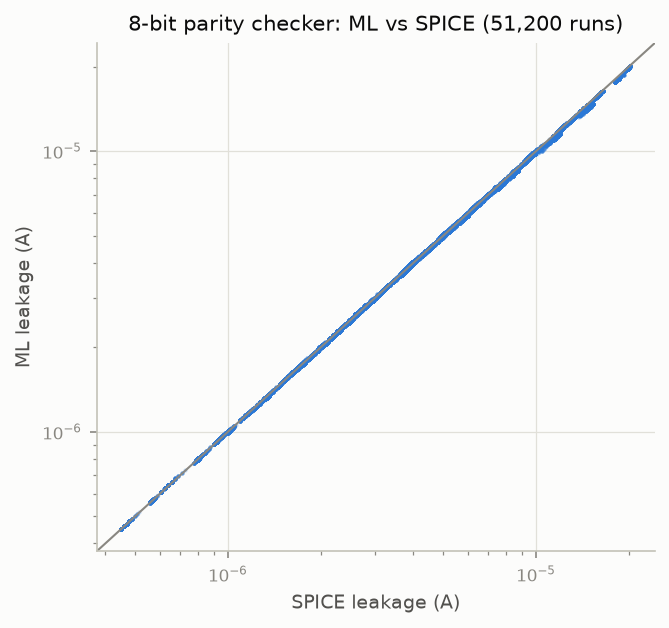
\includegraphics[width=0.5\linewidth]{partC/parity_parity.png}
\caption{Parity checker, ML vs SPICE leakage for all 51,200 runs (log axes).}
\label{fig:paritypar}
\end{figure}

\section{Error Analysis}
\label{sec:errors}

Full numbers are in \file{reports/ERROR_ANALYSIS.md} (\file{scripts/d1_error_analysis.py}).

\paragraph{Transistor models.} The largest relative errors come from four places:
\begin{enumerate}
    \item \textbf{Near-zero currents.} When $|V_d - V_s| < 10$\,mV in an ON device, $I_d$ and $I_s$ are
    tiny differences that can cross zero. The p95 error there is 344\pct\ (NMOS ON), against 0.4\pct\
    at $|V_d - V_s| > 0.5$\,V, but the absolute error is negligible and these currents never enter
    the gate sums.
    \item \textbf{The OFF body current} ($\sim\!10^{-14}$\,A) carries the OFF-case p95 (22\pct\ NMOS,
    20\pct\ PMOS). It is 6--8 decades below the gate leakages, so it does not affect Parts B and C.
    \item \textbf{The mixed-sign OFF terminal} is the hardest real current. Scaling its target by the
    sample's own gate current cut its validation error from 2.84 to 0.96\pct\ median (NMOS OFF) and
    from 4.78 to 1.86\pct\ (PMOS OFF) (\file{scripts/a3c_mixed_scale_study.py}).
    \item \textbf{Corners of the input box.} The median error is nearly flat across temperature,
    \texttt{vth0} and \texttt{toxe}, but the tail grows at the edges, e.g.\ NMOS ON p95 7.2\pct\ at
    $-40$ to $-7$\,\textdegree C against 0.7--1.0\pct\ elsewhere.
\end{enumerate}

\paragraph{Gates and circuit.} The error grows towards the hot and high-$V_{DD}$ corners, where the
leakage is largest or a device sits at the edge of its training range (Figure~\ref{fig:corner}). For
the gates, the median / p95 is 0.46 / 2.5\pct\ at 92--125\,\textdegree C against 0.33--0.38 /
1.0--1.2\pct\ below; for the parity checker 0.75 / 3.4\pct\ against 0.23--0.48 / 0.9--1.2\pct. The
gate error is also higher at the lowest NMOS \texttt{vth0} ($-10$ to $-5$\pct: 0.50\pct\ median) and for
narrow PMOS (45--124\,nm: 0.44 / 2.1\pct\ against 0.31 / 1.0\pct\ for the widest). The
worst corners combine several extremes: corner 168 ($V_{DD} = 0.99$\,V, NMOS \texttt{toxe} $-9.6$\pct,
$W_n = 306$\,nm) and corner 173 (124\,\textdegree C, NMOS \texttt{vth0} $-8$\pct) reach 6.9\pct\ and
6.2\pct\ in single gate cases. There the OFF current exceeds anything in the training data and a tanh
network flattens out; the linear-baseline variant helps most here.

\begin{figure}[H]
\centering
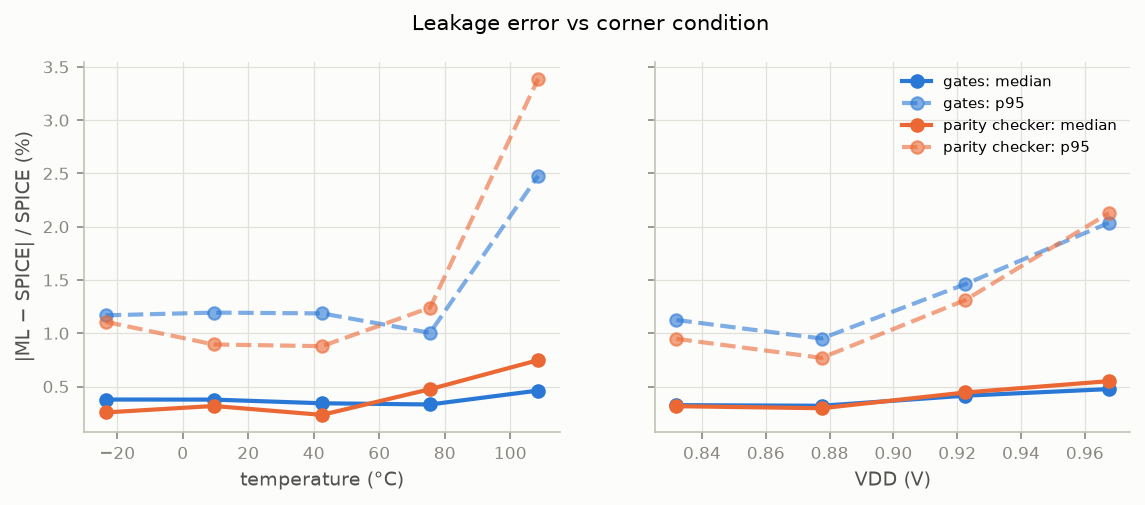
\includegraphics[width=0.85\linewidth]{error_vs_corner.png}
\caption{Median and p95 leakage error vs temperature and $V_{DD}$, for the gates and the parity checker.}
\label{fig:corner}
\end{figure}

\section{Limitations and Improvements}
\label{sec:limits}

\begin{itemize}
    \item \textbf{Edges of the input box.} Gates bias their transistors at the edges of the $(V_d, V_s)$
    square, which uniform sampling covers thinly. Adding 10,000 training rows concentrated there made
    things worse (OFF-case validation median 1.05 $\to$ 2.6\pct, gate median 1.88 $\to$ 2.14\pct), so we
    kept uniform sampling and added more uniform data. A model with physical structure in $V_{ds}$,
    e.g.\ $I \propto 1 - e^{-V_{ds}/v_t}$, would handle the edges better.
    \item \textbf{Joint extremes} (hot + low \texttt{vth0}, or thin oxide + high $V_{DD}$, with a wide
    device) still reach a few percent in single gate cases. A stress set at these corners in the
    selection rule, or denser sampling there, would reduce it.
    \item \textbf{Validation accuracy in the bulk is not enough.} The GP has the best validation median
    (0.07--0.53\pct), but in the gates it gives 12.6\pct\ median error: away from its training points
    an RBF kernel falls back towards the mean, while the MLP extends the trend. This is why we select on
    the p95.
    \item \textbf{Composition from stand-alone gates.} Inside the circuit the gate inputs are up to
    18\,mV off the rails, which leaves 0.18\pct\ median between the sum of SPICE gate values and the
    full circuit.
    \item \textbf{Scope.} One model file, nominal $V_{DD} = 0.9$\,V, DC leakage only. Within a gate or
    circuit all NMOS share one width and all PMOS another; mixed sizings need no new models, only new
    SPICE references.
\end{itemize}

\section{Team Contributions}

We split the work equally, one part each, and each part went into the repository as its own commit
and pull request.

\begin{center}
\begin{tabular}{lp{0.6\linewidth}}
\toprule
Member & Work \\
\midrule
Aryan Agrawal (2023102050) & Simulation setup: the single-transistor ngspice driver
(\file{sim/spec.py}, \file{sim/runner.py}) and its check against the professor's sample netlist.
Part A data: generating the four 10,000-sample datasets, the data check and trend plots. Section~3. \\
\addlinespace
Vansh Jaiswal (2024102013) & Part A models: features and targets, the comparison of the four
techniques, the data-size study, the ensembles and their averages, model selection and the test
results (\file{ml/}, \file{scripts/a3*}, \file{scripts/a4*}). Section~4. The GitHub repository and
the README. \\
\addlinespace
Saarthak Sabharwal (2023102055) & Part B: the gate netlists and SPICE runs, the ML gate leakage with
the cut through the OFF devices, the leakage components and the gate diagnostics
(\file{sim/gates.py}, \file{ml/gate_eval.py}, \file{scripts/b*}). Section~5. \\
\addlinespace
Manikya Pant (2023112024) & Part C: the parity checker netlist and SPICE runs, the ML composition,
the error analysis and the fresh-data check (\file{sim/parity.py}, \file{scripts/c*},
\file{scripts/d1*}, \file{scripts/d3*}). Sections~6--8. Putting the report together. \\
\bottomrule
\end{tabular}
\end{center}

We all wrote parts of the report and checked each other's results. The pull requests were opened from
Vansh's GitHub account and reviewed and merged by the owner of each part.

\section{Conclusion}

Our transistor models, MLP ensembles chosen over a polynomial, LightGBM and a Gaussian process,
predict the four terminal currents of the 45nm\_MGK device to 0.12--0.23\pct\ median test error.
Combined with Kirchhoff's law over a cut through the OFF devices, they give the leakage of the five
gates with a \textbf{0.51\pct\ mean error (99.49\pct\ mean accuracy)} over 3,600 simulations. With
the leakage defined as all current drawn from $V_{DD}$-level sources, the 8-bit parity checker's
leakage is simply the sum of its 28 NAND2 gate leakages, and it reaches the same \textbf{0.51\pct\
mean error} over 51,200 runs. On fresh corners that influenced nothing, the gates and the circuit give
0.50\pct\ and 0.52\pct. The errors that remain are at the joint extremes of the input range, where the
models extrapolate.

\section*{Use of AI Tools}

An AI assistant was used to support parts of this work. We guided it throughout, reviewed and checked
every step and result ourselves, and we take full responsibility for the models, the results and the
report, in line with the responsible use of AI.

\begin{thebibliography}{9}
\bibitem{doc}
Digital VLSI Design, \emph{ML-Driven PVT-Variation-Aware Leakage Estimation}, project document,
IIIT Hyderabad, 2026.
\bibitem{roy}
K.~Roy, S.~Mukhopadhyay and H.~Mahmoodi-Meimand, ``Leakage current mechanisms and leakage reduction
techniques in deep-submicrometer CMOS circuits,'' \emph{Proc.\ IEEE}, vol.~91, no.~2, pp.~305--327, 2003.
\bibitem{weste}
N.~Weste and D.~Harris, \emph{CMOS VLSI Design: A Circuits and Systems Perspective}, 4th ed., Pearson.
\bibitem{bsim4}
BSIM Group, UC Berkeley, \emph{BSIM4 MOSFET Model User's Manual}, \url{https://bsim.berkeley.edu}
\bibitem{ptm}
Predictive Technology Model (PTM), Arizona State University, \url{https://ptm.asu.edu}
\bibitem{ngspice}
ngspice, \url{https://ngspice.sourceforge.io}
\bibitem{sklearn}
F.~Pedregosa et al., ``Scikit-learn: Machine learning in Python,'' \emph{JMLR}, vol.~12, pp.~2825--2830, 2011.
\bibitem{lgbm}
G.~Ke et al., ``LightGBM: A highly efficient gradient boosting decision tree,'' \emph{NeurIPS}, 2017.
\bibitem{gp}
C.~E.~Rasmussen and C.~K.~I.~Williams, \emph{Gaussian Processes for Machine Learning}, MIT Press, 2006.
\end{thebibliography}

\end{document}
